%% Springer Nature (sn-jnl) version of the Native Mamba-2 audit paper.
%% Build: pdflatex main -> bibtex main -> pdflatex main -> pdflatex main
\documentclass[pdflatex,sn-mathphys-num]{sn-jnl}

\usepackage{manyfoot}
\usepackage{amsmath,amssymb}
\usepackage{graphicx}
\usepackage{booktabs}
\usepackage{multirow}
\usepackage{bm}
\usepackage{xcolor}
\usepackage{url}
\usepackage[expansion=false]{microtype}
\usepackage{algorithm}
\usepackage{algpseudocode}

\graphicspath{{figures/}}
\setlength{\emergencystretch}{1.5em}
\renewcommand{\topfraction}{0.9}
\renewcommand{\textfraction}{0.08}
\renewcommand{\floatpagefraction}{0.8}
\raggedbottom

\begin{document}

\title[Continuous-State and Variational Biases in Native Mamba-2]{Dissecting Continuous-State and Variational Inductive Biases in State Space Duality: An Empirical Audit of Native Mamba-2 Cross-Modal Alignment}

\author{\fnm{Madapati Naga Durga} \sur{Abhinav Sai}}\email{abhinav.24bca7148@vitapstudent.ac.in}
\author{\fnm{T V R M} \sur{Siva Shanmukh}}\email{shanmukh.24bce7269@vitapstudent.ac.in}
\author*{\fnm{Rajesh} \sur{Duvvuru}}\email{rajesh.duvvuru@vitap.ac.in}

\affil{\orgdiv{School of Computer Science and Engineering}, \orgname{VIT-AP University}, \orgaddress{\city{Amaravati}, \postcode{522237}, \state{Andhra Pradesh}, \country{India}}}

\abstract{\unboldmath Mamba-2 and its State Space Duality (SSD) scale linearly with sequence length, which makes them tempting replacements for self-attention in vision-language retrieval. Before stacking extra machinery on top of them, though, it is worth asking whether that machinery actually helps. We test three add-ons on frozen ViT-B/16 and RoBERTa-base encoders: a Hamiltonian-inspired dissipative adapter (HEDO) with a skew-symmetric interaction $\mathbf{J}=(\mathbf{A}-\mathbf{A}^\top)/\sqrt{d}$ and positive diagonal damping; Adaptive Variational State Coupling (AVSC), a confidence-gated symmetric KL penalty between vision and text Gaussian posteriors; and Multi-Scale State Aggregation (MSA), which fuses mean, chunk-boundary and terminal states. We ran eight configurations with three seeds each (24 runs) on Flickr8k and compared every variant to a linear-projection baseline using paired 95\% Student-$t$ intervals. Mamba-2 with HEDO was statistically indistinguishable from the baseline (37.31\% vs.\ 37.16\% Mean Recall; $\Delta=+0.15$ pp, CI $[-1.42, +1.73]$) while running at 7,054 pairs/s with 1,086 MB peak memory. MSA cost roughly 10.5 pp, with intervals entirely below zero. AVSC was far worse: every configuration that used it fell to 5.0--6.6\% Mean Recall ($\Delta\approx-31$ pp), a pattern that looks like representation collapse. We argue that matching intermediate posteriors pulls against the repulsive term of the contrastive loss, and we spell out what this implies for anyone building multimodal SSMs.}

\keywords{Cross-modal retrieval, State space models, Mamba-2, Contrastive learning, Hamiltonian dynamics, Variational coupling, Negative results}

\maketitle

%% ============================================================================
\section{Introduction}
\label{sec:intro}

Image-text retrieval asks a model to place pictures and captions in one embedding space so that matching pairs sit close together~\cite{radford2021learning,wang2016comprehensive}. Transformers have done this job well for years~\cite{vaswani2017attention,dosovitskiy2021image,liu2019roberta}, but attention costs $O(L^2)$ in sequence length, and that bill grows quickly with dense patch grids and long captions.

Structured state space models offer a cheaper route. S4~\cite{gu2022efficiently} made long-range recurrence trainable, Mamba~\cite{gu2023mamba} made its parameters input-dependent, and Mamba-2~\cite{dao2024transformers} showed that a selective SSM with scalar decay is the same thing as multiplying by a 1-semiseparable matrix. That observation, called State Space Duality, lets the recurrence run chunk by chunk on tensor cores while keeping $O(L)$ cost.

At the same time, two other ideas have been gaining ground. Physics-inspired networks borrow Hamiltonian structure to keep dynamics stable~\cite{greydanus2019hamiltonian,vanderschaft2000}, and variational bottlenecks are used to smooth latent spaces~\cite{kingma2014auto,alemi2017deep}. It is easy to imagine combining all of these with Mamba-2. It is much harder to find evidence on whether the combination works. Most published variants are tested once, with one seed, and without isolating each component, so a reported gain could come from the SSM, the adapter or plain noise.

We set out to check this carefully. Our question was simple: \emph{do continuous-state adapters and variational coupling improve cross-modal alignment on top of native Mamba-2, or do they break it?} We made four contributions:
\begin{enumerate}
\item We describe HEDO, a dissipative coordinate-momentum adapter placed before native Mamba-2 blocks, and show that its continuous-time energy cannot increase.
\item We built an eight-configuration ablation on frozen ViT-B/16 and RoBERTa-base encoders that covers individual and joint uses of HEDO, Mamba-2, MSA and AVSC.
\item We ran every configuration with three seeds and compared each one with the baseline through paired differences and 95\% Student-$t$ intervals, fixing our decision rules before looking at the numbers.
\item We explain the two failure modes we found: positional asymmetry in MSA ($\approx-10.5$ pp) and a conflict between KL matching and contrastive repulsion in AVSC ($\approx-31$ pp).
\end{enumerate}

%% ============================================================================
\section{Related Work}
\label{sec:related}

\textbf{State space models.} An SSM maps an input $x(t)$ to an output $y(t)$ through a hidden state, $\dot{\mathbf{h}}=\mathbf{A}\mathbf{h}+\mathbf{B}x$ and $y=\mathbf{C}\mathbf{h}+\mathbf{D}x$. S4~\cite{gu2022efficiently} tamed training with HiPPO-based structure for $\mathbf{A}$, and Mamba~\cite{gu2023mamba} let $\mathbf{B}$, $\mathbf{C}$ and the step $\Delta$ depend on the input, so the model can decide what to keep. Mamba-2~\cite{dao2024transformers} writes the whole sequence map as
\begin{equation}
\mathbf{y}=\mathbf{M}\mathbf{x},\qquad M_{ij}=C_i\Big(\textstyle\prod_{k=j+1}^{i}A_k\Big)B_j\quad(i\ge j),
\label{eq:ssd}
\end{equation}
a lower-triangular semiseparable matrix. Blocks of this matrix are computed with matrix multiplies inside chunks and a short recurrence links the chunks.

\textbf{Contrastive retrieval.} Most dual-encoder systems train with InfoNCE~\cite{oord2018representation,chen2020simple,he2020momentum}. Wang and Isola~\cite{wang2020understanding} showed that the loss balances two forces: alignment, which pulls positives together, and uniformity, which spreads everything else over the hypersphere. When uniformity loses, embeddings can fall into a low-dimensional subspace, a failure called dimensional collapse~\cite{jing2022understanding}. Flickr8k~\cite{hodosh2013framing} gives five captions per image, so a multi-positive loss is needed to avoid penalising valid alternative captions.

\textbf{Hamiltonian and variational models.} Hamiltonian neural networks~\cite{greydanus2019hamiltonian} learn an energy $\mathcal{H}(\mathbf{q},\mathbf{p})$ and move along its symplectic gradient. Port-Hamiltonian systems add a damping matrix $\mathbf{R}\succeq0$ so that energy can only decrease~\cite{vanderschaft2000}. Variational methods~\cite{kingma2014auto,alemi2017deep} usually pull posteriors toward $\mathcal{N}(\mathbf{0},\mathbf{I})$. Cross-modal variants drop the fixed prior and instead penalise the divergence between the two modalities' posteriors. How that penalty interacts with a spherical contrastive loss has received little attention, and our results suggest it deserves more.

%% ============================================================================
\section{Problem Setting and Hypotheses}
\label{sec:problem}

Let $\mathcal{D}=\{(\mathbf{I}_i,\mathcal{T}_i)\}_{i=1}^{N}$ be a dataset in which each image $\mathbf{I}_i$ has $K=5$ captions. We learn $f_v(\mathbf{I}),f_t(\mathbf{T})\in\mathbb{S}^{d-1}$ with $d=128$ and score pairs by cosine similarity. To keep backbone learning out of the picture, both encoders are frozen:
\begin{equation}
\mathbf{X}_v=\mathrm{ViT}(\mathbf{I})\in\mathbb{R}^{B\times196\times768},\qquad
\mathbf{X}_t=\mathrm{RoBERTa}(\mathbf{T})\in\mathbb{R}^{B\times L\times768},
\label{eq:frozen}
\end{equation}
where we drop the ViT class token and cap captions at $L\le64$. Together the frozen encoders hold 210,622,696 parameters, so every learned change happens in the small head that follows. Before running anything, we wrote down four hypotheses:
\begin{itemize}
\item $H_1$: Mamba-2 with HEDO raises Mean Recall over the linear baseline.
\item $H_2$: MSA raises Mean Recall.
\item $H_3$: AVSC raises Mean Recall.
\item $H_4$: Sequence modelling adds measurable latency and memory, yet throughput stays practical.
\end{itemize}

%% ============================================================================
\section{Method}
\label{sec:method}

Fig.~\ref{fig:arch} shows the pipeline. Each modality passes through a linear projection, the HEDO adapter, a native Mamba-2 block and a pooling head, and a symmetric multi-positive InfoNCE loss ties the two streams together.

\begin{figure}[t]
\centering
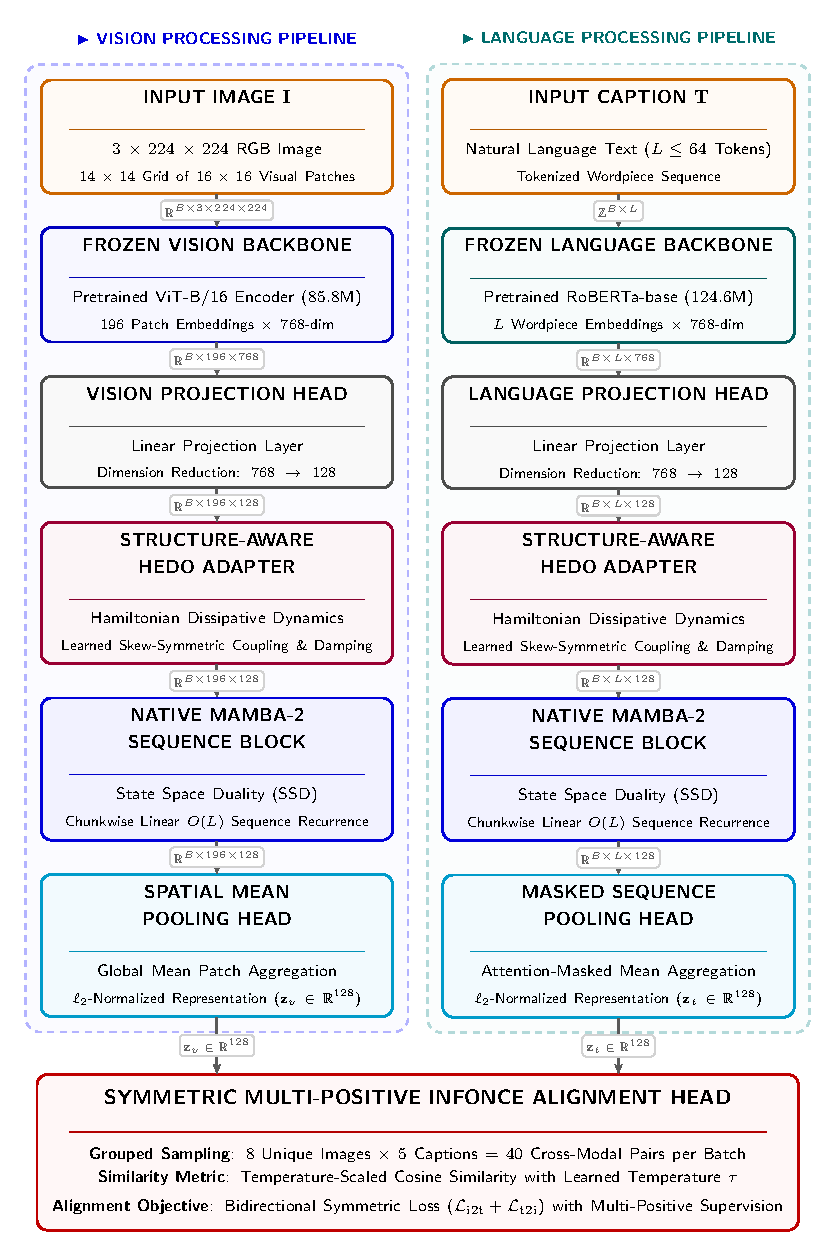
\includegraphics[width=0.7\textwidth]{standalone_architecture.pdf}
\caption{Architecture. Frozen ViT and RoBERTa token features are projected to $d=128$, adapted by HEDO, processed by native Mamba-2 (SSD) blocks, pooled, normalised and aligned with a multi-positive symmetric InfoNCE loss.}
\label{fig:arch}
\end{figure}

\subsection{Projection and baseline}
Both streams are projected with $\mathbf{H}^{(0)}=\mathbf{X}\mathbf{W}$, where $\mathbf{W}\in\mathbb{R}^{768\times128}$ uses Xavier initialisation. In the \texttt{baseline}, these tokens go straight to masked mean pooling and the loss. Because the encoders are frozen, this is the smallest head that can reasonably be used, so any extra module has to earn its place against it.

\subsection{HEDO adapter}
For each token $\mathbf{x}\in\mathbb{R}^d$ we form coordinates and momenta, $\mathbf{q}=\mathbf{W}_q\mathbf{x}$ and $\mathbf{p}=\mathbf{W}_p\mathbf{x}$, and use the quadratic energy $\mathcal{H}=\tfrac12(\|\mathbf{q}\|^2+\|\mathbf{p}\|^2)$. Interactions come from an exactly skew-symmetric matrix and dissipation from a bounded diagonal:
\begin{equation}
\mathbf{J}=\frac{\mathbf{A}-\mathbf{A}^\top}{\sqrt d},\qquad
\mathbf{R}=\mathrm{diag}\big(0.05+0.95\,\sigma(\bm\gamma)\big),
\label{eq:JR}
\end{equation}
with $\mathbf{A}\sim\mathcal{N}(0,0.01^2)$. Hence $\mathbf{v}^\top\mathbf{J}\mathbf{v}=0$ for every $\mathbf{v}$, and each damping entry lies in $[0.05,1]$. The dynamics are
\begin{equation}
\dot{\mathbf{q}}=\mathbf{p}+\mathbf{J}\mathbf{q},\qquad
\dot{\mathbf{p}}=-\mathbf{q}+\mathbf{J}\mathbf{p}-\mathbf{R}\mathbf{p}.
\label{eq:hedo}
\end{equation}

\noindent\textbf{Proposition 1.} \emph{Under \eqref{eq:hedo}, $\dot{\mathcal{H}}=-\mathbf{p}^\top\mathbf{R}\mathbf{p}\le-0.05\|\mathbf{p}\|^2\le0$.}

\noindent\emph{Proof.} $\dot{\mathcal{H}}=\mathbf{q}^\top\dot{\mathbf{q}}+\mathbf{p}^\top\dot{\mathbf{p}}=\mathbf{q}^\top\mathbf{p}+\mathbf{q}^\top\mathbf{J}\mathbf{q}-\mathbf{p}^\top\mathbf{q}+\mathbf{p}^\top\mathbf{J}\mathbf{p}-\mathbf{p}^\top\mathbf{R}\mathbf{p}$. The cross terms cancel and both $\mathbf{J}$ quadratic forms vanish, which leaves $-\mathbf{p}^\top\mathbf{R}\mathbf{p}$. Since $R_{ii}\ge0.05$, the bound follows. $\square$

In practice we take one explicit Euler step with a learned $\Delta t=0.05+0.10\,\sigma(\tau_{\Delta t})\in[0.05,0.15]$. This parameter is separate from the InfoNCE temperature. Proposition~1 applies only in continuous time, since an Euler step carries $O(\Delta t^2)$ error and cannot guarantee that energy drops at every discrete update. We therefore treat the small step and the damping floor as a stabilising bias, not a guarantee, and we check for non-finite values at run time. The output is a small residual,
\begin{equation}
\mathbf{x}_{\mathrm{out}}=\mathbf{x}+0.10\,\mathbf{W}_o\,\mathrm{LayerNorm}(\mathbf{q}_{\mathrm{new}}+\mathbf{p}_{\mathrm{new}}),
\label{eq:hedoout}
\end{equation}
where $\mathbf{W}_o$ uses Xavier initialisation with gain 0.5. As a result, the adapter starts out close to the identity.

\subsection{Native Mamba-2 block}
We use the official \texttt{mamba\_ssm} Mamba-2 module with $d_{\mathrm{model}}=128$, $d_{\mathrm{state}}=64$, $d_{\mathrm{conv}}=4$, an expansion factor of 2, a head dimension of 64 and a chunk size of $Q=16$. The input is widened to 256 channels, passed through a depthwise convolution with kernel size 4, and turned into input-dependent SSM parameters. SSD then produces $\mathbf{Y}\in\mathbb{R}^{B\times L\times128}$.

\subsection{Multi-scale state aggregation (MSA)}
By default we pool with a masked mean, $\bar{\mathbf{y}}_{\mathrm{g}}=\sum_i m_i\mathbf{Y}_i/\sum_i m_i$. MSA adds two more views: the average of chunk-boundary outputs at positions $c_k=\min(kQ,L)-1$, written $\bar{\mathbf{y}}_{\mathrm{b}}$, and the last valid token, written $\mathbf{y}_{\mathrm{last}}$. These are fused as
\begin{equation}
\mathbf{y}_{\mathrm{fused}}=\mathbf{W}_{\mathrm{proj}}\,\mathrm{LayerNorm}\big([\bar{\mathbf{y}}_{\mathrm{g}}\,\|\,\bar{\mathbf{y}}_{\mathrm{b}}\,\|\,\mathbf{y}_{\mathrm{last}}]\big),\qquad \mathbf{W}_{\mathrm{proj}}\in\mathbb{R}^{3d\times d}.
\label{eq:msa}
\end{equation}

\subsection{Adaptive variational state coupling (AVSC)}
Pooled boundary features $\mathbf{h}_v$ and $\mathbf{h}_t$ are mapped to diagonal Gaussians $q_v=\mathcal{N}(\bm\mu_v,\bm\Sigma_v)$ and $q_t=\mathcal{N}(\bm\mu_t,\bm\Sigma_t)$ through linear heads, with $\log\bm\sigma^2$ clamped to $[-6,2]$. The penalty is the symmetric KL divergence
\begin{equation}
\begin{aligned}
\mathcal{D}^{\mathrm{sym}}&=\tfrac12\big(D_{\mathrm{KL}}(q_v\|q_t)+D_{\mathrm{KL}}(q_t\|q_v)\big),\\
D_{\mathrm{KL}}(q_v\|q_t)&=\tfrac12\sum_{k}\Big(\log\tfrac{\sigma_{t,k}^2}{\sigma_{v,k}^2}+\tfrac{\sigma_{v,k}^2+(\mu_{v,k}-\mu_{t,k})^2}{\sigma_{t,k}^2}-1\Big),
\end{aligned}
\label{eq:kl}
\end{equation}
which is weighted per pair by a detached cosine-agreement gate $w_i\in[0,1]$:
\begin{equation}
\mathcal{L}_{\mathrm{KL}}=\lambda_{\mathrm{KL}}\,\tfrac1B\textstyle\sum_i w_i\,\mathcal{D}^{\mathrm{sym}}_i,\qquad \lambda_{\mathrm{KL}}=10^{-3}.
\end{equation}
AVSC acts only during training. At test time, each encoder runs on its own and is deterministic.

\subsection{Training objective}
A grouped sampler draws 8 images together with all 5 of their captions, which gives 40 captions per batch. With logits $S_{ij}=e^{\tau}\,\mathbf{z}_{v,i}^\top\mathbf{z}_{t,j}$, where $\tau$ is initialised to $\log(1/0.07)$, and with $\mathcal{P}(i)$ denoting the five captions of image $i$ and $i^*(j)$ the parent image of caption $j$,
\begin{equation}
\mathcal{L}_{i2t}=-\frac18\sum_{i=1}^{8}\frac{1}{5}\sum_{j\in\mathcal{P}(i)}\log\frac{e^{S_{ij}}}{\sum_{k=1}^{40}e^{S_{ik}}},\qquad
\mathcal{L}_{t2i}=-\frac1{40}\sum_{j=1}^{40}\log\frac{e^{S_{i^*(j)j}}}{\sum_{i=1}^{8}e^{S_{ij}}},
\label{eq:nce}
\end{equation}
and the total loss is $\mathcal{L}=\tfrac12(\mathcal{L}_{i2t}+\mathcal{L}_{t2i})+\mathcal{L}_{\mathrm{KL}}$. The KL term is present only when AVSC is switched on. Gradients are clipped at norm 1.0 and parameters are updated with AdamW.



%% ============================================================================
\section{Experimental Setup}
\label{sec:setup}

\textbf{Data and training.} We use the standard Flickr8k split~\cite{hodosh2013framing}: 6,000 training, 1,000 validation and 1,000 test images, each with five captions. Images are resized to $224\times224$ and normalised with ImageNet statistics, and captions go through the RoBERTa tokenizer and are cut at 64 tokens. Each model trains for 10 epochs with AdamW at a learning rate of $10^{-4}$, a weight decay of $10^{-4}$ and a gradient-clipping threshold of 1.0.

\textbf{Configurations.} Four binary switches give $2^4=16$ possible models, and we trained the eight listed in Table~\ref{tab:cfg}. These eight do not form a full factorial design. For example, we did not run Mamba-2 without HEDO or MSA on its own. The full model is best read as a stress test of how the modules behave together, not as the design we expected to win.

\begin{table}[t]
\centering
\caption{The eight ablation configurations.}
\label{tab:cfg}
\begin{tabular}{lcccc}
\toprule
Configuration & HEDO & Mamba-2 & MSA & AVSC\\
\midrule
\texttt{baseline} & -- & -- & -- & -- \\
\texttt{mamba2\_hedo} & \checkmark & \checkmark & -- & -- \\
\texttt{mamba2\_msa} & -- & \checkmark & \checkmark & -- \\
\texttt{hedo\_msa} & \checkmark & -- & \checkmark & -- \\
\texttt{avsc\_msa} & -- & -- & \checkmark & \checkmark \\
\texttt{mamba2\_avsc} & -- & \checkmark & -- & \checkmark \\
\texttt{full\_model} & \checkmark & \checkmark & \checkmark & \checkmark \\
\texttt{hedo\_avsc} & \checkmark & -- & -- & \checkmark \\
\bottomrule
\end{tabular}
\end{table}

\textbf{Metrics.} On the 1,000-image test set we report R@1, R@5 and R@10 in both directions, the median rank (MedR), and Mean Recall (MR), which is the average of the six recall values.

\textbf{Statistics.} For each configuration $c$ and seed $s\in\{42,43,44\}$ we compute the paired difference $\Delta_{c,s}=\mathrm{MR}_{c,s}-\mathrm{MR}_{\mathrm{base},s}$ and form the interval $\bar\Delta_c\pm t_{0.025,2}\,s_c/\sqrt3$, where $t_{0.025,2}=4.303$. We decided on the reading rule in advance. An interval entirely above zero counts as \emph{supported}, one that contains zero means \emph{no statistical difference}, and one entirely below zero counts as \emph{contradicted}. We report seven comparisons without multiplicity correction. Every run checks that all tensors stay finite and that the official Mamba-2 CUDA kernels are loaded.



%% ============================================================================
\section{Results}
\label{sec:results}

\begin{table}[t]
\centering
\caption{Retrieval on the Flickr8k test set (mean over 3 seeds; MR also shows $\pm$ SD). Recall values are in \%.}
\label{tab:main}
\setlength{\tabcolsep}{3.5pt}
\begin{tabular}{lcccccccrr}
\toprule
& \multicolumn{3}{c}{Image$\to$Text} & \multicolumn{3}{c}{Text$\to$Image} & & \multicolumn{2}{c}{MedR}\\
\cmidrule(lr){2-4}\cmidrule(lr){5-7}\cmidrule(lr){9-10}
Configuration & R@1 & R@5 & R@10 & R@1 & R@5 & R@10 & MR & i2t & t2i\\
\midrule
Baseline & 16.53 & 43.27 & \textbf{57.47} & 13.92 & \textbf{38.31} & \textbf{53.45} & $37.16\pm0.57$ & 7.7 & 9.0\\
Mamba-2 + HEDO & \textbf{17.40} & \textbf{43.47} & 57.20 & \textbf{14.20} & 38.25 & 53.35 & $\mathbf{37.31\pm0.68}$ & 7.7 & 9.0\\
\midrule
Mamba-2 + MSA & 9.77 & 29.53 & 42.90 & 8.92 & 28.22 & 41.98 & $26.89\pm0.68$ & 13.8 & 14.7\\
HEDO + MSA & 9.47 & 29.50 & 42.87 & 8.33 & 27.45 & 40.84 & $26.41\pm0.49$ & 14.7 & 15.3\\
\midrule
AVSC + MSA & 1.47 & 6.40 & 11.50 & 1.50 & 6.51 & 12.48 & $6.64\pm0.82$ & 81.7 & 61.3\\
Mamba-2 + AVSC & 1.80 & 6.27 & 11.87 & 1.05 & 5.55 & 10.19 & $6.12\pm1.14$ & 99.8 & 72.3\\
Full model & 1.47 & 5.97 & 10.73 & 1.25 & 5.60 & 10.69 & $5.95\pm0.42$ & 94.3 & 69.7\\
HEDO + AVSC & 1.03 & 4.93 & 9.27 & 1.01 & 4.83 & 9.20 & $5.04\pm0.84$ & 103.2 & 79.0\\
\bottomrule
\end{tabular}
\end{table}

\begin{figure}[t]
\centering

\includegraphics[width=0.75\textwidth]{fig_factorial_recall.pdf}
\caption{Recall@1/5/10 for (a) image-to-text and (b) text-to-image retrieval. Error bars show $\pm1$ SD over three seeds. The configurations fall into three clear groups.}
\label{fig:recall}
\end{figure}

\subsection{Overall picture}
Table~\ref{tab:main} and Fig.~\ref{fig:recall} show three distinct groups. The baseline and Mamba-2 + HEDO lie close together at about 37\% MR. The two MSA models land near 26--27\%. All four models that include AVSC end up between 5\% and 7\%. The same ordering holds at every recall cutoff and in both retrieval directions.

\subsection{HEDO with Mamba-2 ($H_1$)}
Mamba-2 + HEDO reaches $37.31\pm0.68\%$ MR, with R@1 of 17.40\% for image-to-text and 14.20\% for text-to-image. It is slightly ahead of the baseline on R@1, but the paired difference is only $+0.15$ pp and its interval, $[-1.42, +1.73]$, includes zero (Table~\ref{tab:delta}). $H_1$ is therefore not supported. The safer reading is that the adapter and the SSM block keep baseline accuracy and do not cause instability. They do not add accuracy.

\subsection{MSA ($H_2$)}
Adding boundary and terminal states hurts. Mamba-2 + MSA drops by $10.27$ pp (CI $[-13.10,-7.44]$) and HEDO + MSA by $10.75$ pp (CI $[-12.38,-9.12]$). Both intervals lie entirely below zero, so $H_2$ is contradicted.

\subsection{AVSC ($H_3$)}
AVSC produced the largest effect in the study, and the effect was negative. Every configuration that used it lost between 30.5 and 32.1 pp. R@1 fell to 1--2\%, and median rank rose from 8--9 to between 61 and 103. The full model, which combines all four modules, scores $5.95\%$. Whatever HEDO or Mamba-2 might contribute is swamped by the variational term. $H_3$ is contradicted.

\begin{table}[t]
\centering
\caption{Paired Mean Recall differences against the baseline ($n=3$ paired seeds).}
\label{tab:delta}
\setlength{\tabcolsep}{4pt}
\begin{tabular}{lcccl}
\toprule
Comparison & $\Delta$ per seed (42/43/44) & Mean $\Delta$ & 95\% CI & Verdict\\
\midrule
Mamba-2 + HEDO & $-0.27/-0.15/+0.88$ & $+0.15$ & $[-1.42,+1.73]$ & No diff.\\
Mamba-2 + MSA & $-11.26/-9.02/-10.53$ & $-10.27$ & $[-13.10,-7.44]$ & Worse\\
HEDO + MSA & $-11.12/-9.99/-11.14$ & $-10.75$ & $[-12.38,-9.12]$ & Worse\\
AVSC + MSA & $-31.01/-30.94/-29.60$ & $-30.52$ & $[-32.49,-28.54]$ & Worse\\
Mamba-2 + AVSC & $-32.98/-29.83/-30.30$ & $-31.04$ & $[-35.26,-26.81]$ & Worse\\
Full model & $-31.55/-30.56/-31.51$ & $-31.21$ & $[-32.60,-29.81]$ & Worse\\
HEDO + AVSC & $-33.71/-31.05/-31.58$ & $-32.11$ & $[-35.61,-28.62]$ & Worse\\
\bottomrule
\end{tabular}
\end{table}



Across seeds, the seed-to-seed spread is small (SD $\le0.68$ pp for the two leading models). However, three seeds give limited power, so the one interval that includes zero should not be taken as proof that the two models are equivalent.

\subsection{Efficiency ($H_4$)}
Table~\ref{tab:eff} and Fig.~\ref{fig:eff} report cost. Mamba-2 + HEDO adds 132,610 trainable parameters. That is 28.5\% more than the baseline head but only 0.063\% of the full model, because the backbones are frozen. Peak memory grows by 43.8 MB (4.2\%), head latency goes from 4.19 to 5.67 ms, and end-to-end latency goes from 7.64 to 8.39 ms. Throughput stays at 7,054 pairs/s for the head and 4,766 pairs/s end to end, which supports $H_4$. Among the eight models, Mamba-2 + HEDO lies on the accuracy-throughput Pareto front. The MSA and AVSC variants cost more and give worse accuracy.

\begin{table}[t]
\centering
\caption{Cost of each configuration (mean over 3 seeds; p/s = pairs per second).}
\label{tab:eff}
\setlength{\tabcolsep}{4pt}
\begin{tabular}{lrrrrrr}
\toprule
Configuration & Params & VRAM (MB) & Train (s) & Lat.\ (ms) & Head p/s & E2E p/s\\
\midrule
Baseline & 465,177 & 1,042.31 & 278.4 & 4.19 & 9,550 & 5,240\\
Mamba-2 + HEDO & 597,787 & 1,086.15 & 362.8 & 5.67 & 7,054 & 4,766\\
Mamba-2 + MSA & 565,273 & 1,045.36 & 306.3 & 4.49 & 8,916 & 5,089\\
HEDO + MSA & 697,883 & 1,088.07 & 399.0 & 5.80 & 6,902 & 4,419\\
AVSC + MSA & 631,321 & 1,046.63 & 367.3 & 5.70 & 7,029 & 4,355\\
Mamba-2 + AVSC & 531,225 & 1,043.18 & 329.8 & 5.16 & 7,774 & 4,718\\
Full model & 763,931 & 1,089.33 & 463.1 & 7.07 & 5,671 & 3,749\\
HEDO + AVSC & 663,835 & 1,087.42 & 427.7 & 6.16 & 6,501 & 4,112\\
\bottomrule
\end{tabular}
\end{table}

\begin{figure}[t]
\centering

\includegraphics[width=0.7\textwidth]{fig_efficiency_tradeoff.pdf}
\caption{(a) Head throughput against Mean Recall. (b) End-to-end throughput against peak training memory. Bubble area is proportional to the number of trainable parameters.}
\label{fig:eff}
\end{figure}

%% ============================================================================
\section{Discussion}
\label{sec:discussion}

\subsection{Why HEDO does no harm}
Three design choices explain why HEDO stays harmless. First, $\mathbf{J}$ is exactly skew-symmetric, so in continuous time it rotates the state without adding energy. Second, the damping floor of 0.05 means energy keeps decreasing in the continuous model (Proposition~1). With small Euler steps, we saw no blow-ups in any of the runs. Third, the 0.10 residual scale keeps the adapter close to the identity, so the geometry learned by the frozen encoders is left largely intact. The flip side is that a module this gentle may not change enough to help, which fits the near-zero difference we measured.

\subsection{Why MSA hurts}
We see two likely causes, and both relate to where the extra states come from. Consider the recurrence $\mathbf{h}_t=\mathbf{A}_t\mathbf{h}_{t-1}+\mathbf{B}_t\mathbf{x}_t$. Its last output is biased toward recent tokens. In an image, the last token is simply the bottom-right patch of the $14\times14$ grid. In a caption, it is whatever word happens to come last. Adding that vector to the embedding brings in a positional bias that has nothing to do with meaning. Chunk-boundary states cause a similar problem, because they sample the recurrence every 16 tokens, and objects and phrases do not line up with those cuts. The masked mean, in contrast, gives equal weight to every contextualised token and is indifferent to order, which suits a symmetric retrieval task. We should be clear that this is an explanation of the results and not something we tested directly.

\subsection{Why AVSC fails}
The two losses act on different parts of the network. InfoNCE works on the final normalised embeddings. Its repulsive gradient on anchor $\mathbf{z}_i$,
\begin{equation}
\nabla_{\mathbf{z}_i}\mathcal{L}_{\mathrm{rep}}=\sum_{j\in\mathcal{N}(i)}\frac{\exp(\tau\mathbf{z}_i^\top\mathbf{z}_j)}{\sum_k\exp(\tau\mathbf{z}_i^\top\mathbf{z}_k)}\,\tau\mathbf{z}_j,
\label{eq:rep}
\end{equation}
pushes non-matching items apart and spreads the embeddings over the sphere~\cite{wang2020understanding}. The symmetric KL term works earlier in the network. It asks the vision and text posteriors to agree in both mean and variance, whatever the other 39 captions in the batch look like. Contrastive learning needs to keep the small differences that separate one candidate from another, and the KL term shrinks exactly those differences. Under our settings ($\lambda_{\mathrm{KL}}=10^{-3}$, log-variance clamp $[-6,2]$), this conflict coincides with the collapse of retrieval.

We are careful about how far this argument goes. An R@1 of 1--2\% and median ranks between 61 and 103 are what collapse would look like. However, we did not track singular-value spectra or effective rank during training, so we cannot claim that the symmetric KL term alone causes dimensional collapse. Measuring those spectra is the obvious next experiment.

\subsection{Practical guidance}
Our results suggest three rules. (i) For retrieval, pool over all tokens and avoid terminal or chunk-boundary states. (ii) Do not add a cross-modal KL term on intermediate features next to a spherical InfoNCE head unless you have evidence that it helps in your setting, because in ours it destroyed retrieval. (iii) If you use a physics-inspired adapter, build in exact skew-symmetry and strictly positive damping. These properties cost little and kept every one of our runs stable.

\subsection{Limitations}
This study covers one small dataset (Flickr8k), frozen encoders, one Mamba-2 size ($d_{\mathrm{model}}=128$, $d_{\mathrm{state}}=64$, $Q=16$), and three seeds per configuration. Each of these limits how widely the findings can be applied. The eight configurations are a subset of the 16 possible ones, so some effects of individual modules remain entangled. We also did not correct for multiple comparisons, although the negative results are large enough that a correction would not change their verdicts. Testing on MS-COCO, fine-tuning the encoders, using more seeds and measuring embedding rank directly would all strengthen the conclusions.

%% ============================================================================
\section{Conclusion}
\label{sec:conclusion}

We tested whether a Hamiltonian-style adapter, multi-scale state pooling and variational cross-modal coupling help native Mamba-2 align images and text. Over 24 runs on Flickr8k, Mamba-2 with HEDO matched a linear baseline (37.31\% vs.\ 37.16\% MR, CI $[-1.42,+1.73]$ pp) at 7,054 pairs/s and 1,086 MB. MSA lowered Mean Recall by about 10.5 pp, and AVSC by about 31 pp. The MSA loss appears to come from positional bias in recurrent states. The AVSC loss fits a conflict between intermediate distribution matching and contrastive repulsion, although direct spectral measurements are still needed to confirm collapse. For anyone putting state space models into multimodal systems, the main message is simple: keep the pooling plain, be cautious with variational coupling, and test every added module against a strong baseline before trusting it.

\backmatter

\bmhead{Acknowledgements}
We thank the maintainers of the open-source \texttt{mamba\_ssm} and \texttt{transformers} libraries.

\section*{Declarations}
\textbf{Funding} No external funding was received for this work.
\textbf{Competing interests} The authors declare no competing interests.
\textbf{Data availability} Flickr8k is publicly available. Code and run logs are available from the corresponding author on reasonable request.

\bibliography{references}

\end{document}
